\documentclass{article}
\usepackage{graphicx} % Required for inserting images
\usepackage{geometry}
\usepackage{circuitikz}
\usepackage{siunitx}
\usepackage{CJKutf8}
\usepackage{amsmath}
\usepackage{amssymb}
\usepackage{caption}
\usepackage{float}
\usepackage{subcaption}
\geometry{top=10mm, left=20mm, a4paper}
\title{Operational Amplifier Circuits Report}
\author{梁程捷(B11901136),吳奕娃(B11901080)}
\date{}

\begin{document}
\begin{CJK*}{UTF8}{bkai}
\maketitle

%============Inverting OP-amp====================
\section*{Inverting OP-Amp Circuit}
\begin{minipage}{0.5\textwidth}
\begin{table}[H]
\begin{tabular}{|c|c|c||c|c|c|}
    \hline
    $f$ (\unit{\kilo\hertz}) &  $V_i$ (V)& $V_o$ (V) & $f$ (\unit{\hertz}) &  $V_i$ (V)& $V_o$ (V)\\
    \hline\hline
    1	& 3.92 & 7.84 & 46  & 4.00 & 5.84   \\
    5   & 3.92 & 7.84 & 47  & 4.00 & 5.68  \\
    10	& 4.00 & 7.84 & 48  & 4.00 & 5.56   \\
    15	& 4.00 & 7.92 & 50  & 4.08 & 5.36   \\
    20	& 4.00 & 7.76 & 60  & 4.00 & 4.56   \\
    25	& 3.92 & 7.68 & 80  & 4.08 & 3.44   \\
    30	& 4.00 & 7.68 & 100 & 4.00 & 2.80   \\
    40	& 4.08 & 6.56 &     &      &        \\

 \hline
\end{tabular}
\caption{inverting op-amp raw experimental data}
\end{table}
\end{minipage}\hspace{20mm}
\begin{minipage}{0.5\textwidth}
    \begin{figure}[H]    
        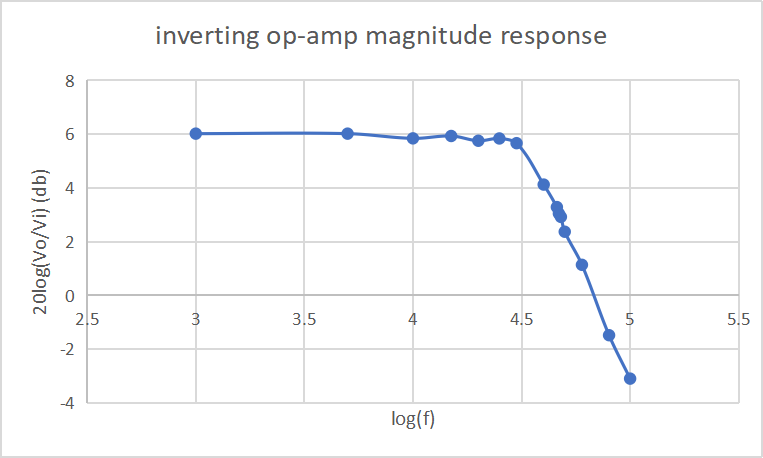
\includegraphics[scale=0.30]{inv_op_amp.png}
        \caption{inverting op-amp magnitude response}
    \end{figure}
\end{minipage}


\begin{minipage}{0.50\textwidth}
    \begin{figure}[H]
        \begin{center}   
            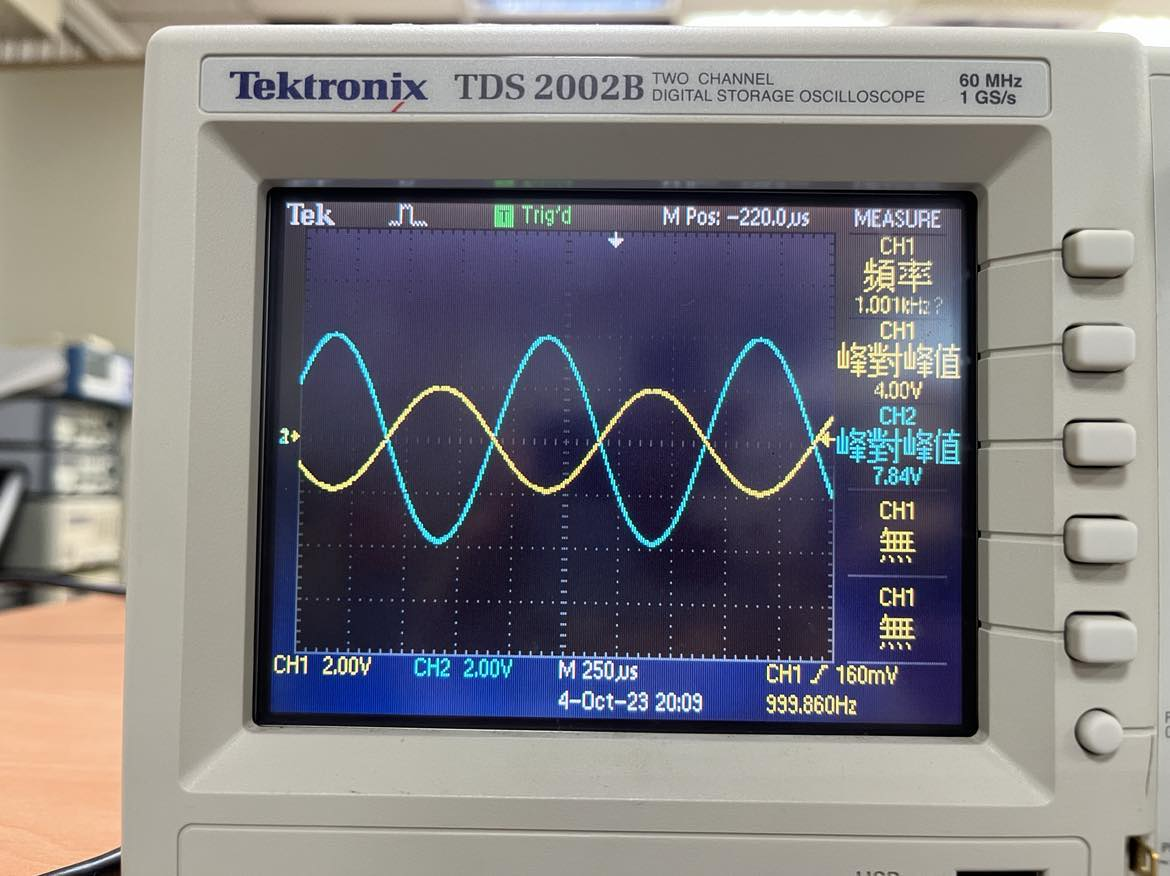
\includegraphics[scale=0.15]{inv_1k.jpg}
            \caption{inverting op-amp input and output \\waveforms}
        \end{center}
    \end{figure}    
\end{minipage}
\begin{minipage}{0.50\textwidth}
    \begin{figure}[H]
        \begin{center}   
            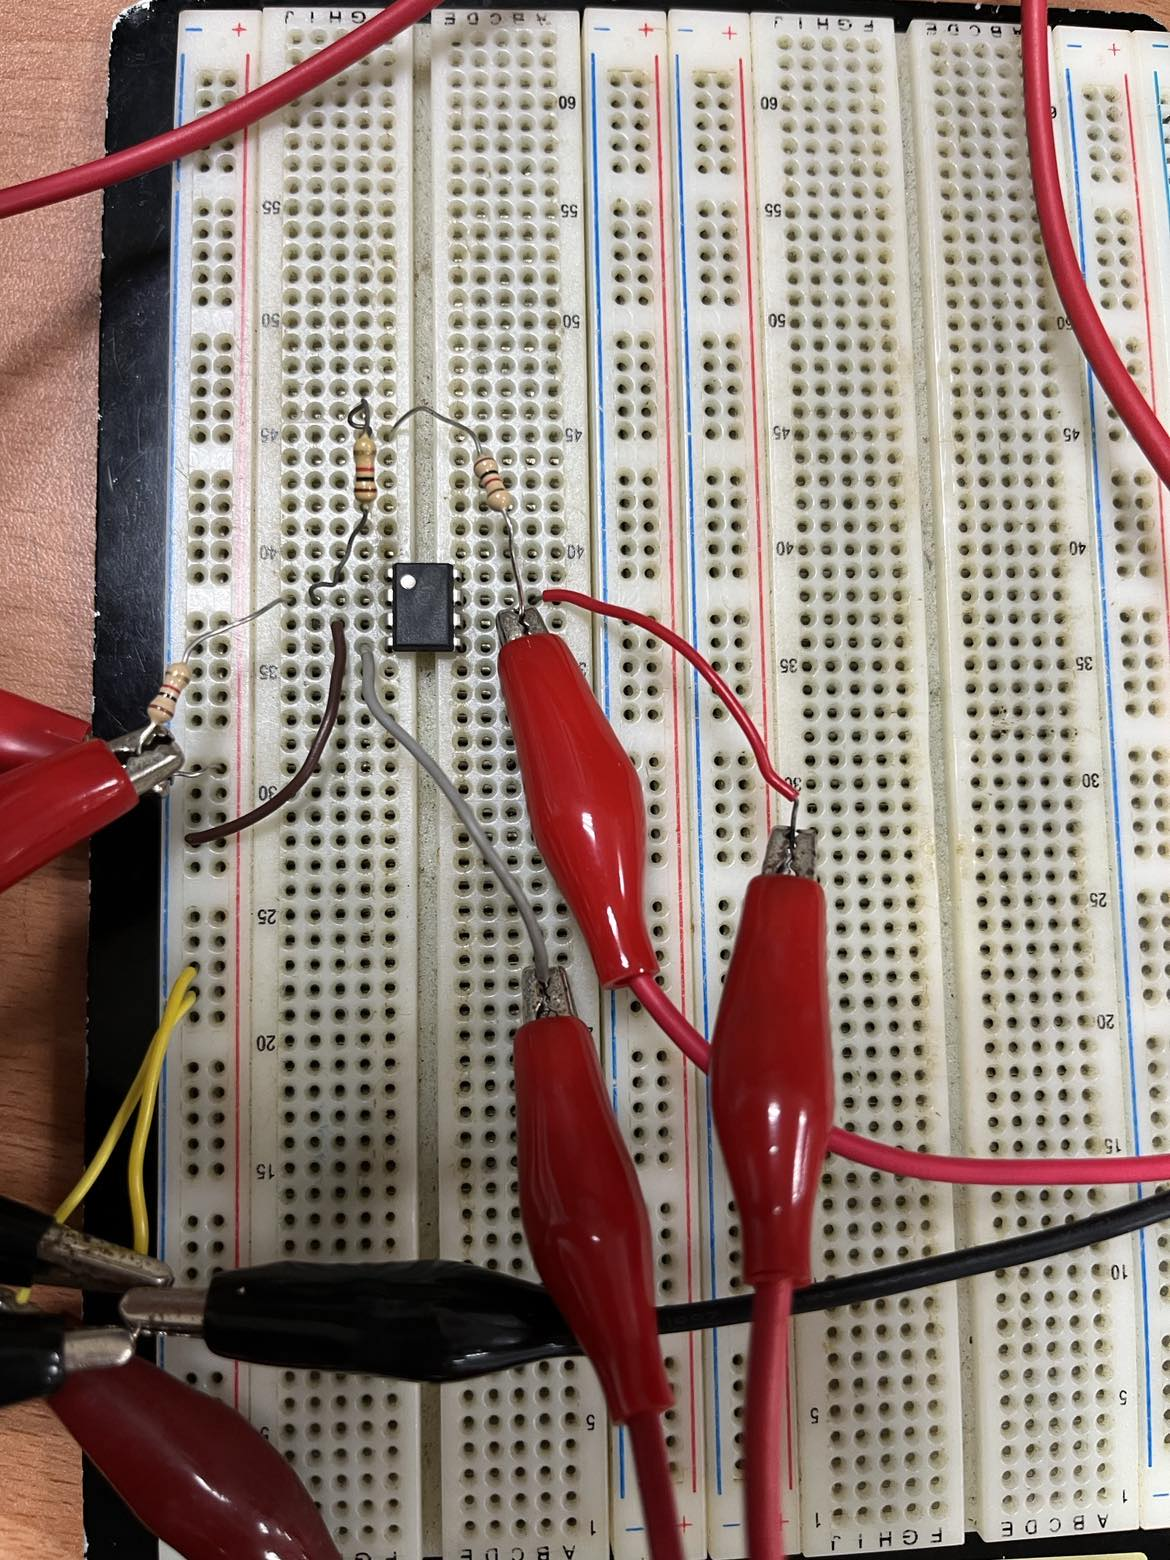
\includegraphics[scale=0.10]{inv_op_amp_circuit.jpg}
            \caption{inverting op-amp circuit}
        \end{center}
    \end{figure}    
\end{minipage}


\begin{center}
\begin{figure}[h]
    
    \begin{subfigure}[b]{0.3\textwidth}
        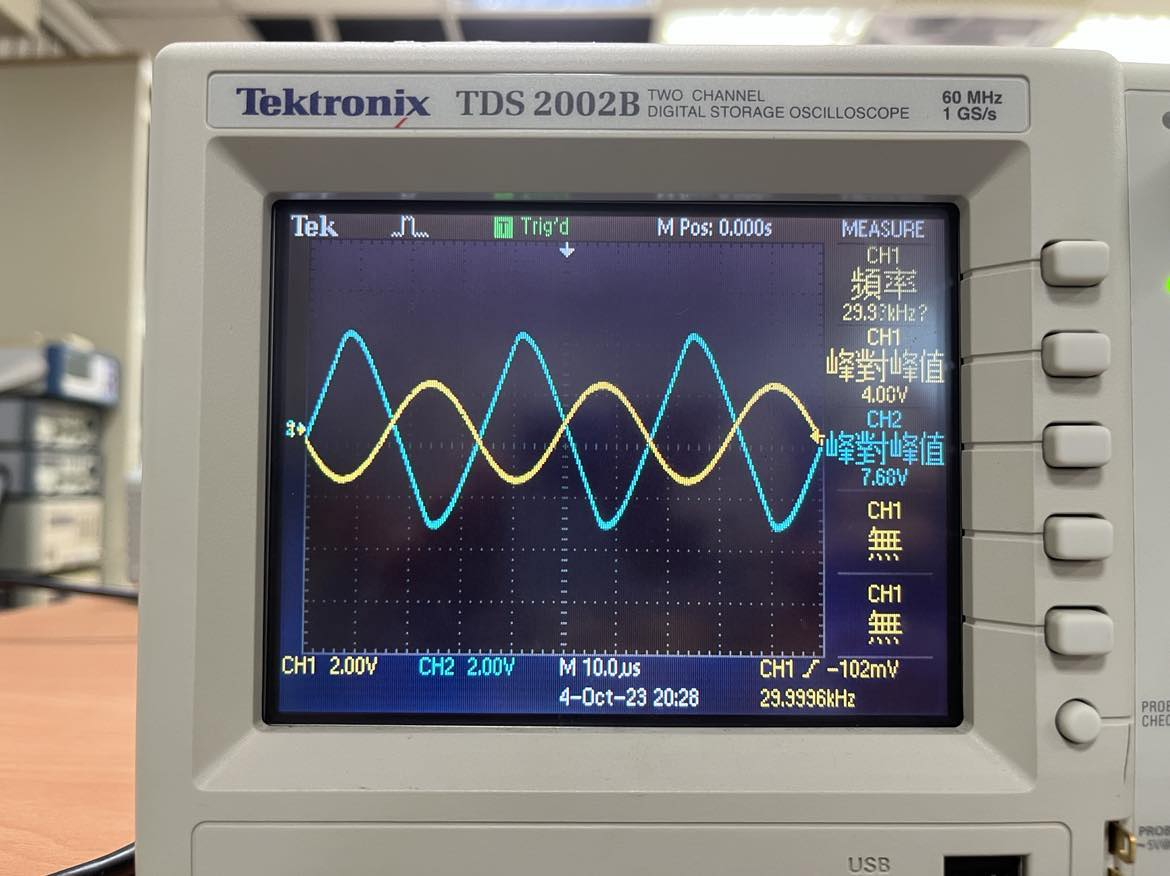
\includegraphics[width=\textwidth]{inv_30k.jpg}
        \caption{$f = 30$ \unit{\kilo\hertz}}
    \end{subfigure}
    ~
    \begin{subfigure}[b]{0.3\textwidth}
        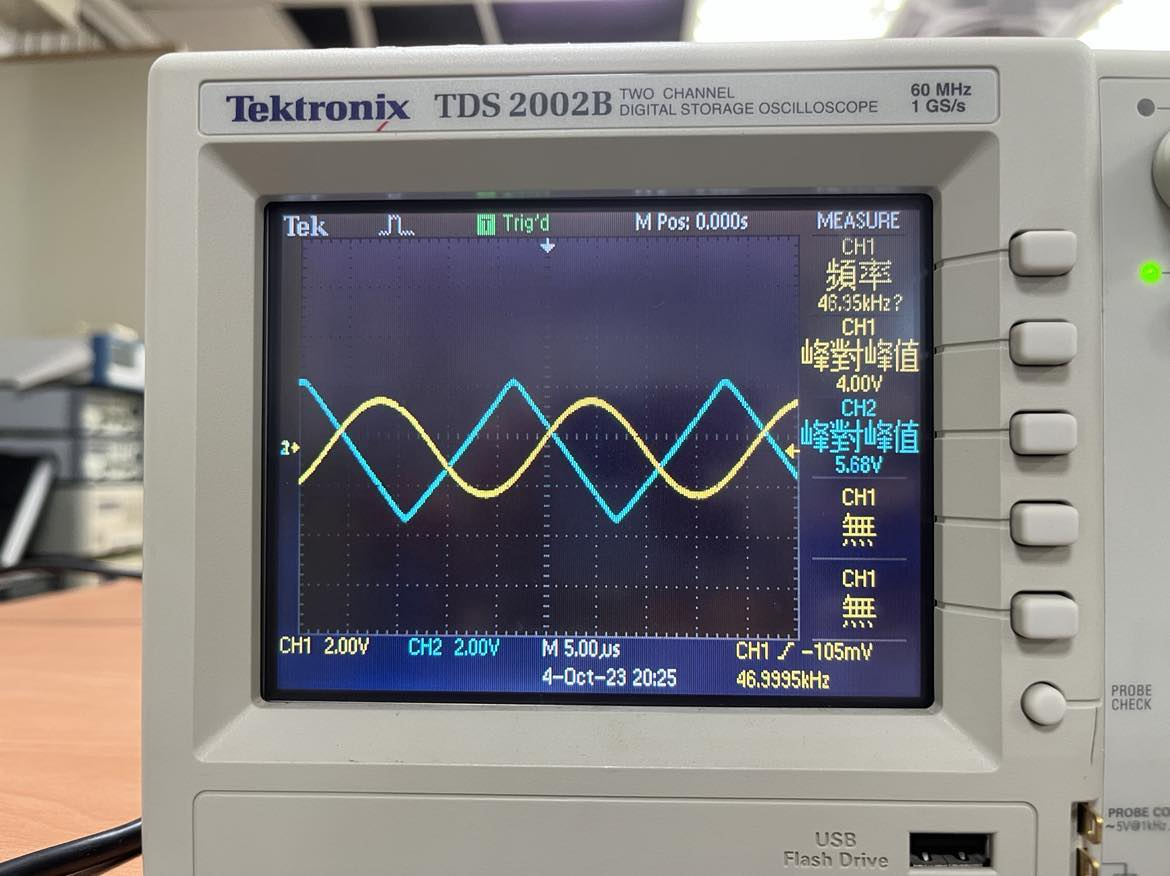
\includegraphics[width=\textwidth]{inv_47k.jpg}
        \caption{$f = 47$ \unit{\kilo\hertz}}
    \end{subfigure}
    ~
    \begin{subfigure}[b]{0.3\textwidth}
        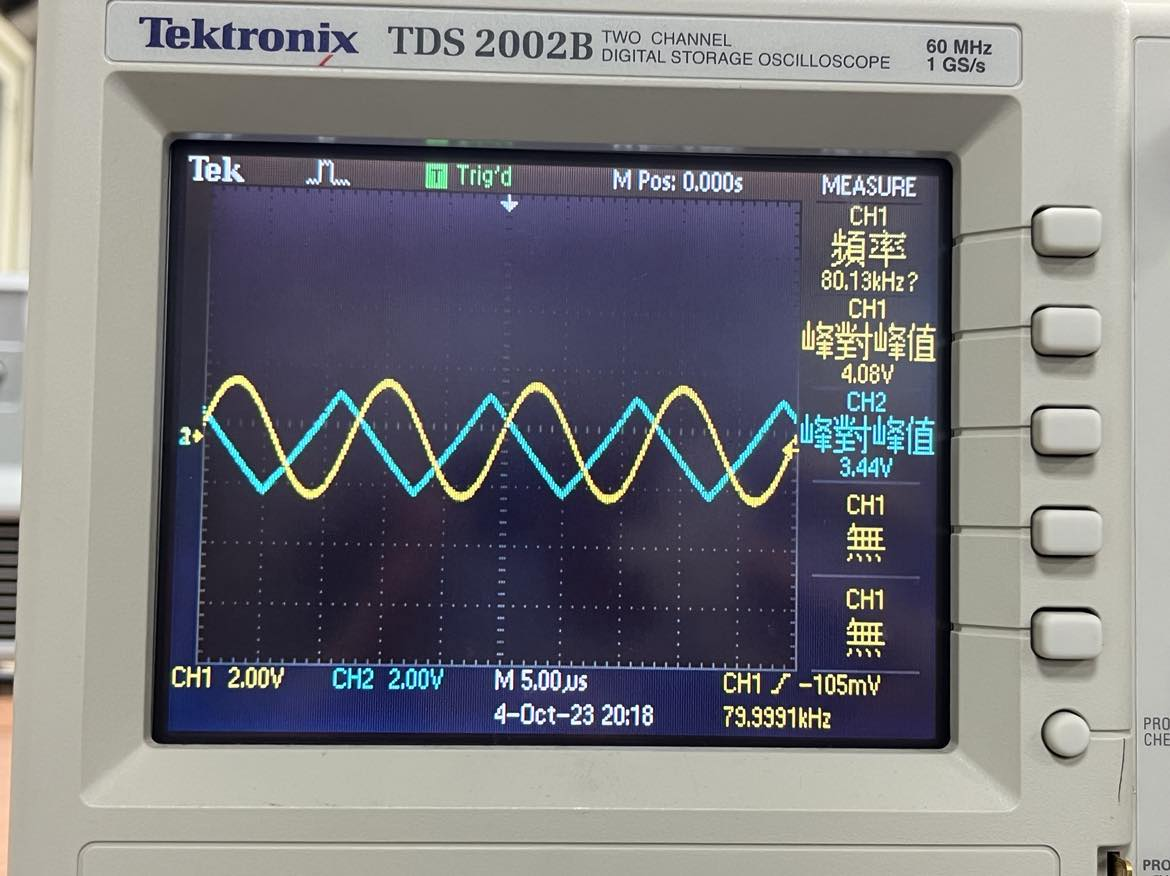
\includegraphics[width=\textwidth]{inv_80k.jpg}
        \caption{$f = 80$ \unit{\kilo\hertz}}
    \end{subfigure}
\end{figure}
\end{center}

\textbf{As shown in the figure, there is a phase shift occured in this circuit.}
\begin{equation*}
    \text{Measured } f_{3dB} = 47 \text{ \unit{\kilo\hertz}}
\end{equation*}



%============Non-inverting OP-amp====================
\section*{Non-Inverting OP-Amp Circuit}

\begin{minipage}{0.45\textwidth}
\begin{table}[H]
\begin{tabular}{|c|c|c||c|c|c|}
    \hline
    $f$ (\unit{\kilo\hertz}) &  $V_i$ (V)& $V_o$ (V) & $f$ (\unit{\kilo\hertz}) &  $V_i$ (V)& $V_o$ (V)\\
    \hline\hline
    0.5	& 4.08 & 12.4 & 32  & 4.08 & 8.00   \\
    1   & 4.20 & 12.4 & 35  & 4.08 & 7.44   \\
    20	& 4.16 & 12.0 & 40  & 4.16 & 6.88   \\
    21	& 4.08 & 11.6 & 100 & 4.16 & 2.84   \\
    22	& 4.08 & 11.2 & 200 & 4.08 & 1.40   \\
    25	& 4.08 & 10.4 & 300 & 4.08 & 1.00   \\
    27	& 4.08 & 9.60 & 400 & 4.08 & 0.74   \\
    28	& 4.08 & 9.28 & 500 & 4.08 & 0.62   \\
    30	& 4.08 & 8.64 &     &      &        \\
 \hline
\end{tabular}
\caption{non-inverting op-amp raw experimental data}
\end{table}    
\end{minipage}\hspace{25mm}
\begin{minipage}{0.45\textwidth}
\begin{figure}[H]
    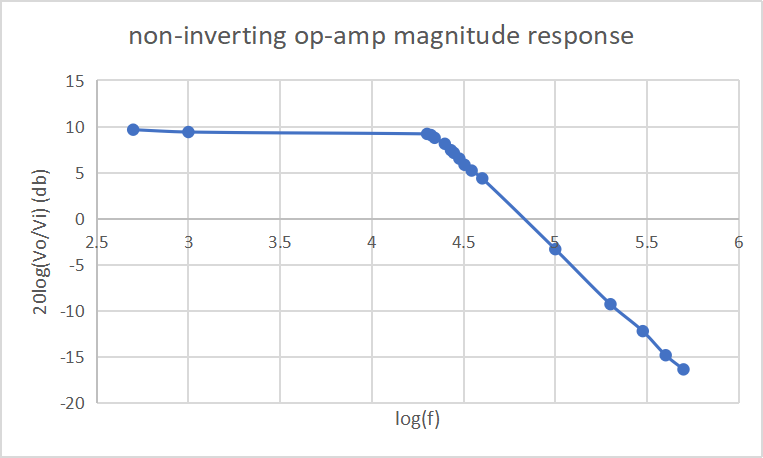
\includegraphics[scale=0.30]{noninv_op_amp.png}
    \caption{non-inverting op-amp magnitude response}
\end{figure}
\end{minipage}

\begin{minipage}{0.50\textwidth}
    \begin{figure}[H]
        \begin{center}   
            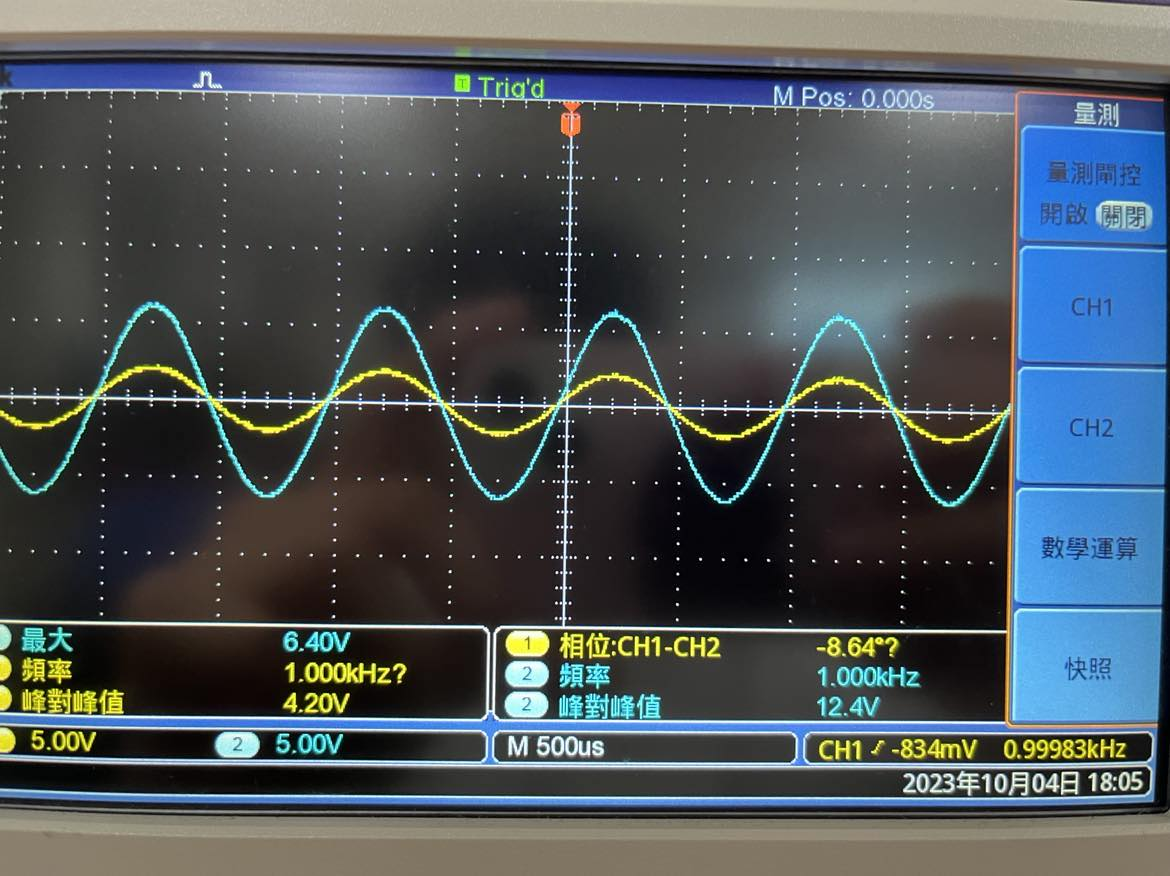
\includegraphics[scale=0.15]{noninv_1k.jpg}
            \caption{non-inverting op-amp input and output \\waveforms}
        \end{center}
    \end{figure}    
\end{minipage}
\begin{minipage}{0.50\textwidth}
    \begin{figure}[H]
        \begin{center}   
            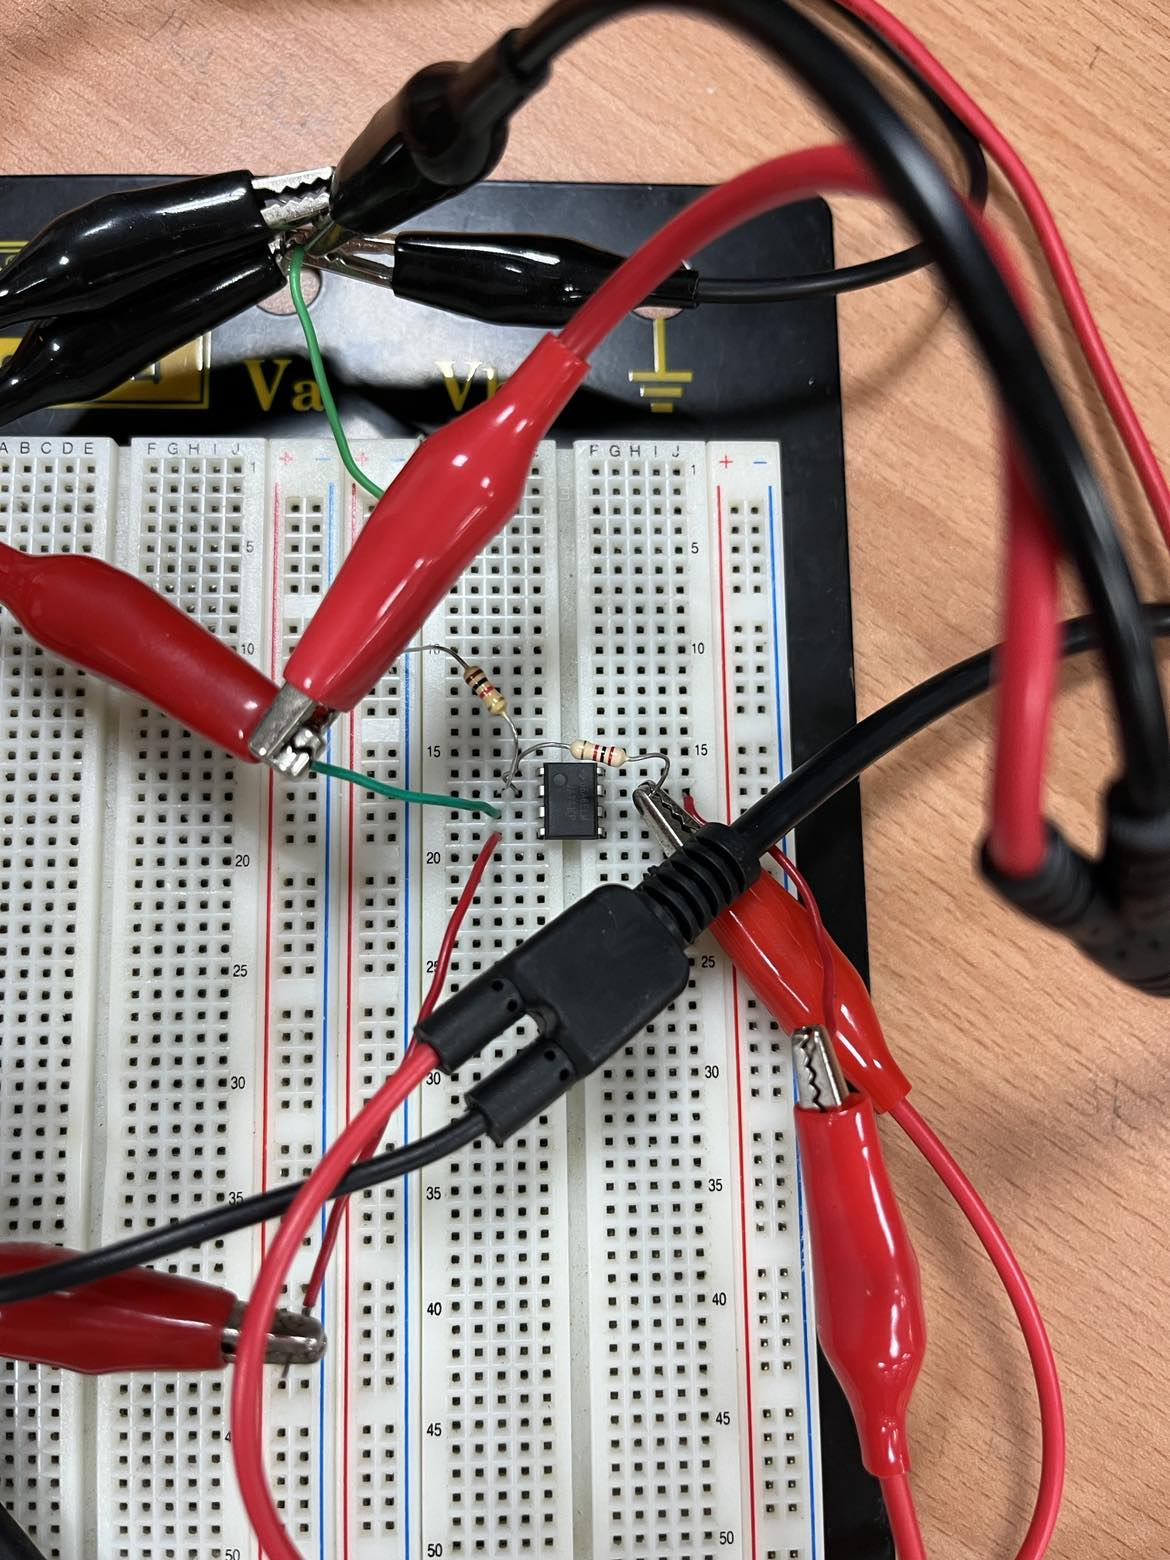
\includegraphics[scale=0.10]{noninv_op_amp_circuit.jpg}
            \caption{non-inverting op-amp circuit}
        \end{center}
    \end{figure}    
\end{minipage}


\begin{center}
\begin{figure}[h]
    
    \begin{subfigure}[b]{0.3\textwidth}
        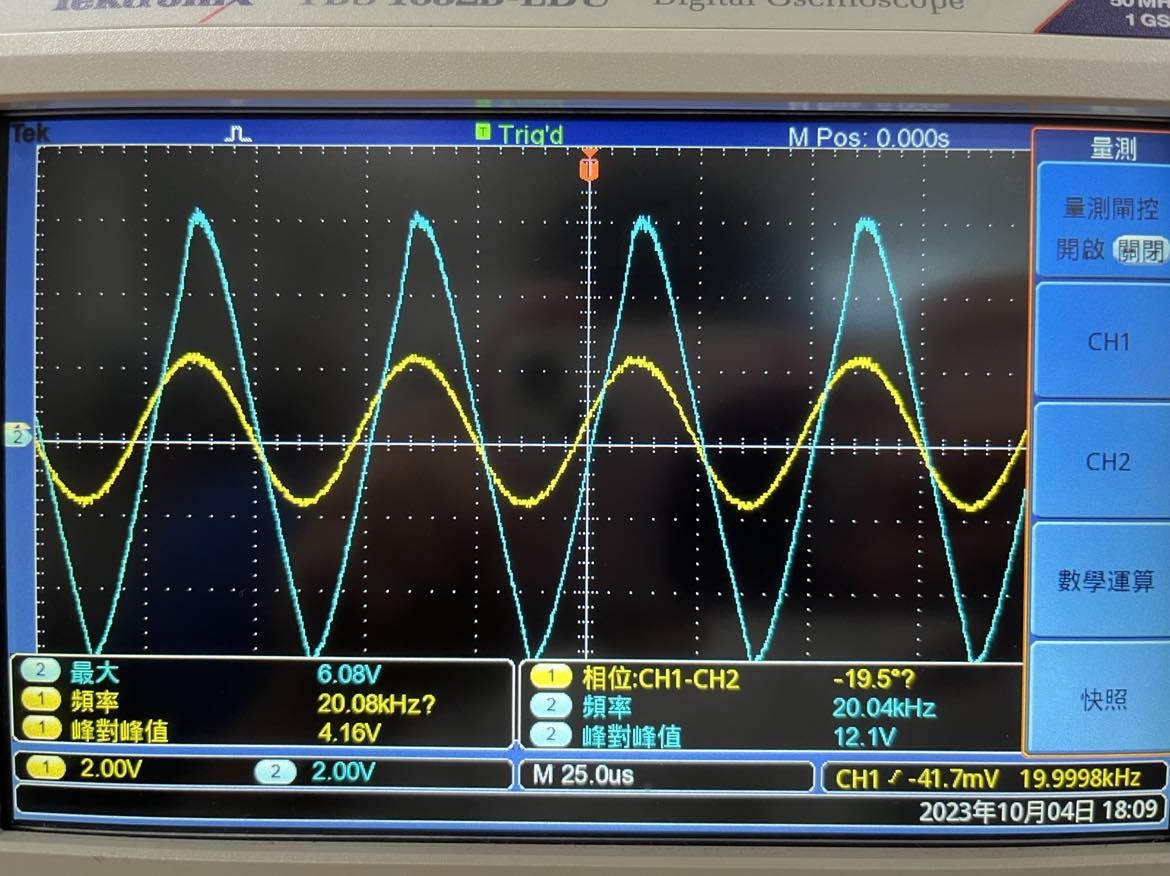
\includegraphics[width=\textwidth]{noninv_20k.jpg}
        \caption{$f = 20$ \unit{\kilo\hertz}}
    \end{subfigure}
    ~
    \begin{subfigure}[b]{0.3\textwidth}
        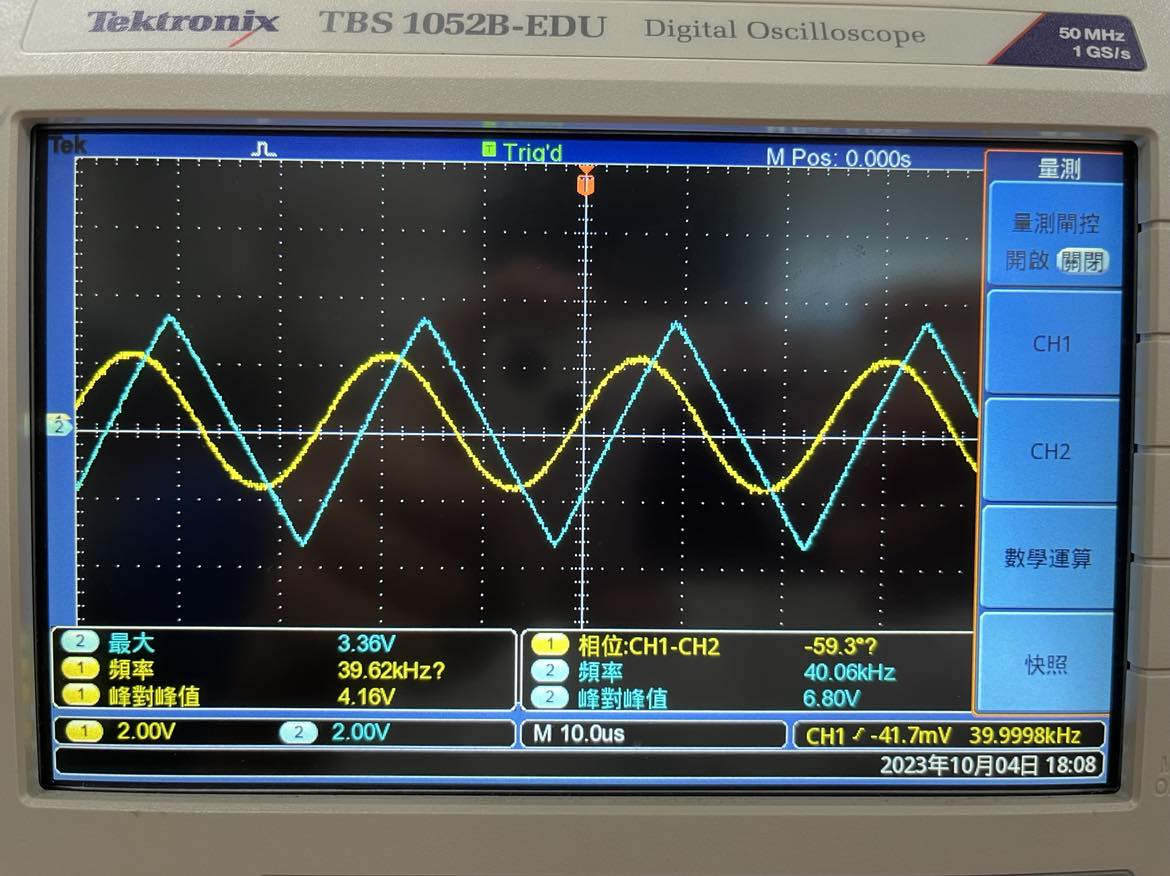
\includegraphics[width=\textwidth]{noninv_40k.jpg}
        \caption{$f = 40$ \unit{\kilo\hertz}}
    \end{subfigure}
    ~
    \begin{subfigure}[b]{0.3\textwidth}
        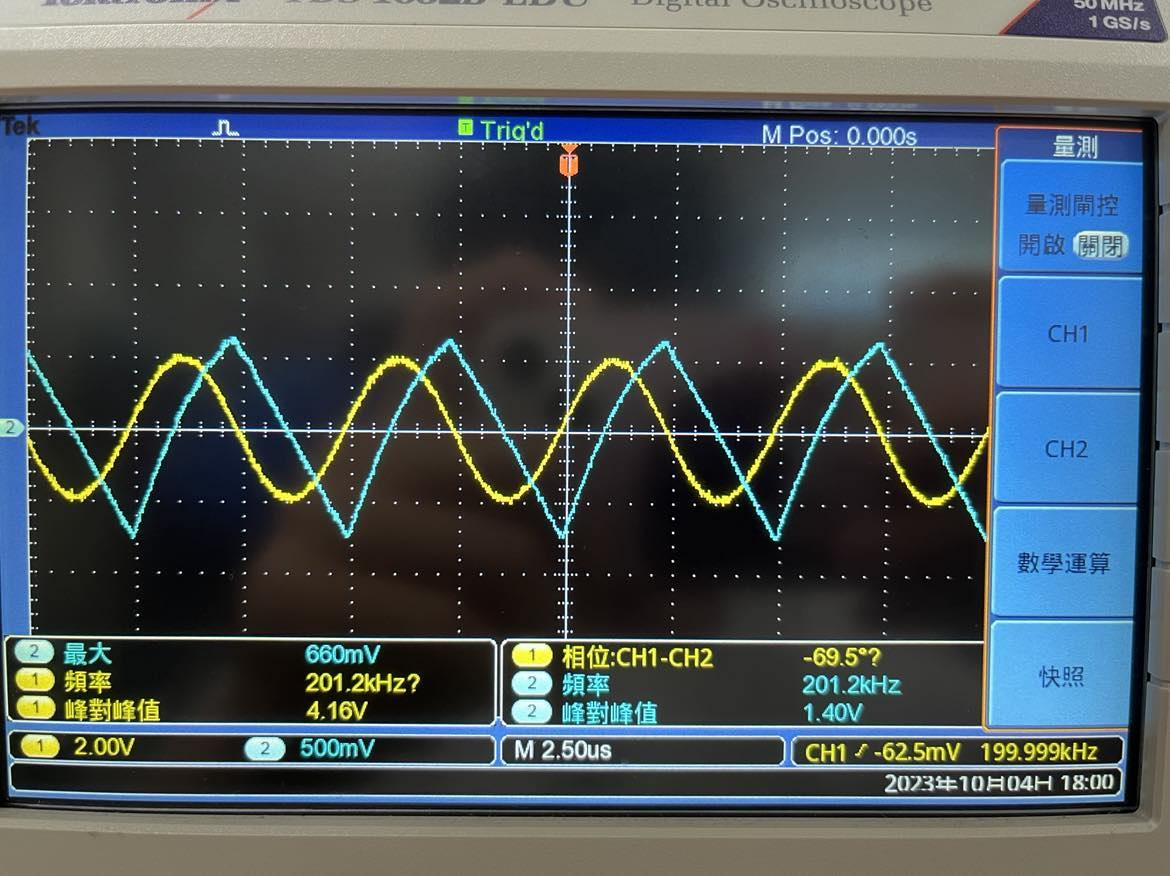
\includegraphics[width=\textwidth]{noninv_200k.jpg}
        \caption{$f = 200$ \unit{\kilo\hertz}}
    \end{subfigure}
\end{figure}
\end{center}

\textbf{As shown in the figure, there is a phase shift occured in this circuit.}
\begin{equation*}
    \text{Measured } f_{3dB} = 30 \text{ \unit{\kilo\hertz}}
\end{equation*}

\end{CJK*}
\end{document}
